\documentclass[a4paper,12pt]{article}
\parindent 0pt
\parskip 1mm
\usepackage[dvips]{epsfig}
\usepackage{url}

\begin{document}

\begin{center}
{\Large\bf CN 510 - Principles and Methods of Cognitive and Neural Modeling}

\bigskip

{\large\bf Assignment \# 3}
\smallskip

{\large\bf John Joseph}
\end{center}

\bigskip
{\bf Replicating the Izhikevich Neuron}
\bigskip

This assignment asks us to replicate twenty differnet firing patters using the Izhikevich model of the neuron. The neuron potential is modelled using a differential equation that evolves two variables, $V$ and $u$, with time. 

\begin{equation}
\frac{dV}{dt} = 0.04V^{2}+5V+140-u+I
\end{equation}
\begin{equation}
\frac{du}{dt} = a(bV-u)
\end{equation}

The equation is controlled by parameters $I$ (our input current), $a$, and $b$, as well as the initial conditions $V_{0}$ and $u_{0}$. Additionally, there are two further parameters $c$ and $d$ that manage the spiking conditions once our potential crosses a certain threshold. 

\vspace{2mm}

This brings the number of parameters left to the user up to 8 ($I, a, b, c, d, V_{0}$, $u_{0}, V_{spike}$). Adjusting these parameters causes the model to exhibit several different firing patterns. This report will demonstrate my attempts at recreating twenty firing patterns outlined by Izhikevich. This was accompished with varying degrees of success, and the final results seem to reflect two things: the sensitivity and complexity of this model, and my inexperience as a programmer. 

\vspace{2mm}

The simulations were run twice for 200 seconds each using a time step of 1 second and a time step of 0.1 second. My general strategy was to use the input settings provided in the assignment and, when I found the output to be significantly different from the output produced by Izhikevich, toyed with the parameters until I felt I could do no more. For the record, I ran the simulation using the two aforementioned timesteps separately using the Euler method and the Runge-Kutta 4 method. I pick and chose which of these four possible outcomes to use in this report, all for the sake of neatness and accuracy when compared to Izhikevich. 
\vspace{2mm}

Each firing pattern will be given a page in this report, in which I will provide a plot of its output and a short description of my process in creating it. 

\vfil\eject

{\bf Results}

\vspace{2mm}

{\bf Tonic Spiking}
\bigskip

The first pattern is the Tonic Spiking pattern, characterized by a constant spiking period following the application of an input current, set to a constant 14 (amps, presumably) starting at 10s. 

\vspace{2mm}

The implementation of this pattern was extremely straightforward. For future reference the $c$ value means the voltage will reset to $c$ once it has passed our $vSpike$ value, which was set to 30 in all cases. Similarly, $u$ will be set to $u+d$ post spike.

\vspace{2mm}

Parameters: $a=0.02, b=0.2, c=-50, d=2, I=15, $

\vspace{1mm}

$V=_{0}=-70, u_{0}=-20$. 

\begin{figure}[h!]
\begin{center}
\epsfig{file=data/figures/A,width=14cm,height=8cm}
\end{center}
\caption{\label{pict1}Tonic Spiking Voltage, with $I$ in blue}
\end{figure}

Though I can't really account for spike amplitude, I will say that this plot does seem to follow Izhikevich's quite well; note the constant spiking period the neuron converges to following the application of I. 

\vspace{2mm}

Notice the inital spike during the first 10ms; this is something I could never really account for, and it shows up in many of the upcoming simulations. I tried several initial conditions

\vfil\eject

{\bf Phasic Spiking}
\bigskip

The second pattern is Phasic Spiking, meaning we get a quick spike followed by a period of inactivity. 

\vspace{2mm}

Parameters: $a=0.02, b=0.2, c=-50, d=2, I=15, $

\vspace{1mm}

$V=_{0}=-70, u_{0}=-20$. 

\begin{figure}[h!]
\begin{center}
\epsfig{file=data/figures/B,width=14cm,height=8cm}
\end{center}
\caption{\label{pict2}Phasic Spiking Voltage, with $I$ in blue}
\end{figure}

Note the relatively small application of current; this is perhaps the biggest differentiator between the phasic and tonic modes, and it seems to me that this input current is not sufficient to send the neuron into a constant spiking state. 

\vfil\eject


{\bf Tonic Bursting}
\bigskip

We now simulate Tonic Bursting, which is similar to Tonic Spiking in that it maintains a constant period, but differs in its rapid bursts of spikes rather than constant single spikes.

\vspace{2mm}

Parameters: $a=0.02, b=0.2, c=-50, d=2, I=15, $

\vspace{1mm}

$V=_{0}=-70, u_{0}=-20$. 

\begin{figure}[h!]
\begin{center}
\epsfig{file=data/figures/C,width=14cm,height=8cm}
\end{center}
\caption{\label{pict3}Tonic Bursting Voltage, with $I$ in blue}
\end{figure}

It is here that I should point out the initial weirdness I got in most of my tests; at t=0 I often got some strange spiking behavior. I could negate this by changing the initial conditions, though in some cases (like this one) I couldn't quite shake it. 

\vspace{2mm}

Also, I chose to use a smaller timestep for this example (DT=0.1) because I found it helped to localize the bursts. All plots will be included in the final report. 

\vfil\eject

{\bf Phasic Bursting}
\bigskip

The Phasic Bursting pattern is similar to the Phasic spiking, save for a rapid succession of spikes rather than just one. Implementation was very straightforward, and I did not run into any sort of issues for this pattern

\vspace{2mm}

Parameters: $a=0.02, b=0.25, c=-55, d=0.05, I=0.6, $

\vspace{1mm}

$V_{0}=-70, u_{0}=-20$. 

\begin{figure}[h!]
\begin{center}
\epsfig{file=data/figures/D,width=14cm,height=8cm}
\end{center}
\caption{\label{pict4}Phasic Bursting Voltage, with $I$ in blue}
\end{figure}

One thing I couldn't quite seem to lock down was the localization of the spikes; I had wanted a pattern in which the bursts were in much more rapid succession. My thinking was to vary $u$, which did work to a degree. 

\vspace{2mm}

I resolved this in the previous example by using a smaller time step, but for the Phasic Spiking pattern this actually had the opposite effect. 

\vfil\eject

{\bf Mixed Mode}
\bigskip

Part 5 asked us to simulate a neuron firing in a Mixed Mode pattern. In general, a Mixed Mode oscillation is a pattern that exhibits oscillations shifting between faster and slower periods and differing amplitudes.

\vspace{2mm}

Looking at the output, I do think that it is very close to what Izhikevich obtained. However, I don't really see a mixed mode pattern in either of our outputs, unless we are considering the initial burst state to have shifted to the slower spiking state it eventually reaches once $t=200$. 
\vspace{2mm} 

Parameters: $a=0.02, b=0.2, c=-55, d=4, I=10, $

\vspace{1mm}

$V_{0}=-70, u_{0}=-20$. 

\begin{figure}[h!]
\begin{center}
\epsfig{file=data/figures/E,width=14cm,height=8cm}
\end{center}
\caption{\label{pict5}Mixed Mode, with $I$ in blue}
\end{figure}

I mentioned before that I usually got some during the very early stages of my simulation, so I wasn't sure if that initial burst was due to error on my part or the accuracy of the simulation.

\url{http://math.bu.edu/people/tasso/Chaos_18_015101.pdf}

\vfil\eject

{\bf Spike Frequency Adaptation}
\bigskip

The next firing pattern was called Spike Frequency Adaptation. An article I found by Wilanowski and Piotrkiewicz defines the pattern as the decline in firing rate of a neuron in response to a constant current input; in other words, the application of a relatively large current otherwise capable of generating wild spiking patterns becomes depolarized to a more predictable stable spiking state. 

\vspace{2mm}

Parameters: $a=0.01, b=0.2, c=-65, d=8, I=30, $

\vspace{1mm}

$V_{0}=-70, u_{0}=-20$. 

\begin{figure}[h!]
\begin{center}
\epsfig{file=data/figures/F,width=14cm,height=8cm}
\end{center}
\caption{\label{pict6}Spike Frequency Adaptation, with $I$ in blue}
\end{figure}

To me, this looks like the output of the Mixed Mode oscillation. However, front he current overlay you can see that a much larger current has been applied, meaning the neuron was able to stabilize itself and produce a neat spiking pattern. I chose to use the smaller timestep of DT=0.1 in this example, as I found it made the output and initial burt look a bit more neat. 

\url{http://www.frontiersin.org/Cellular_Neuroscience/10.3389/fncel.2012.00050/full}

\vfil\eject

{\bf Class 1 Excitability}
\bigskip

It is here that I began to run into some hiccups in my simulations. Class 1 excitability is defined by Izhikevich to be an input-dependent spiking mode, meaning the spiking frequency scales directly with the amount of input current being applied. 

\vspace{2mm} 

Parameters: $a=0.02, b=-0.1, c=-55, d=6, I=0.5t, $

\vspace{1mm}

$V_{0}=-70, u_{0}=0$. 

\begin{figure}[h!]
\begin{center}
\epsfig{file=data/figures/G,width=14cm,height=8cm}
\end{center}
\caption{\label{pict7}Class 1 Excitability, with $I$ in blue}
\end{figure}

With sufficient applications of current, one does see the firing rate increase the amount of current applied goes up. The slope of that line is 0.5, meaning it's value at $t=100$ is 50 amps. Tests with slopes greater than 1 were carried out, and an increase in firing rate was observed; $DT$ in Class 1 and 2 = 0.1

\vspace{2mm}

This is to be expected for Class 1, but as you will see in Class 2 I think this is indicative of a larger problem. 

\vfil\eject

{\bf Class 2 Excitability}
\bigskip

As opposed to the input-dependent frequency of Class 1 excitable neurons, Class 2 neurons should exhibit a constant spiking frequency regardless of the applied voltage. 

\vspace{2mm}

However, in my actual plot of the data I found this system to be very sensitive to input currents; the amount of current $I$ eventually applied in this model was significantly lower than the current applied to the Class 1 neuron, and yet the spiking frequency was quick to blow up. It was tough to say whether or not the actual rate increased during the 200 second run, but the fact remains that the spike period was dramatically lower once the current was increased. 
 
\vspace{2mm} 

Parameters: $a=0.2, b=0.26, c=-65, d=0, I=0.05t, $

\vspace{1mm}

$V_{0}=-70, u_{0}=0$. 

\begin{figure}[h!]
\begin{center}
\epsfig{file=data/figures/H,width=14cm,height=8cm}
\end{center}
\caption{\label{pict8}Class 2 Excitability, with $I$ in blue}
\end{figure}

\url{ftp://ftp-sop.inria.fr/athena/Team/Olivier.Faugeras/ArticlesCoursENS-MVA/izhikevich-nesb.pdf}

\vfil\eject

{\bf Spike Latency}
\bigskip

The spike latency pattern is characterized by a single spike, preceded by a short delay following the application of an input current. 

\vspace{2mm}

Though it is small, there is an apparent ``slowing down'' of the voltage spike just before it hits its peak voltage. This effect appears more pronounced in Izhikevich's diagram, though that could have been fore demonstrational purposes. To accentuate my dip I chose $DT=0.1$ in this output. 
 
\vspace{2mm} 

Parameters: $a=0.05, b=0.26, c=-60, d=0, I=2, $

\vspace{1mm}

$V_{0}=-25, u_{0}=-20$. 

\begin{figure}[h!]
\begin{center}
\epsfig{file=data/figures/I,width=14cm,height=8cm}
\end{center}
\caption{\label{pict9}Spike Latency, with $I$ in blue}
\end{figure}

Something I will touch upon several times in this report was my inability to really control the rapidity of the firing patterns. In particular, I feel that this pattern looks ``rushed''; I would have preferred the spike latency period to have been more spread out. 

\vspace{2mm}

However, I think the overall shape is indicative of a latency pattern, and I consider this simulation a success. 

\vfil\eject

{\bf Sub-Threshold Oscillations}
\bigskip

This firing pattern is characterized by the genration of a small oscillation in the voltage pattern, one not strong enough to generate a spike and reset but still strong enough to be evident. 

\vspace{2mm}

For the record, I chose to plot this data using my Runge-Kutta data; this is a rare thing for me to do in this report, but in this case I thought the oscillations looked a bit smoother using this method rather than Euler. The Euler plot was very similar, save for some sharp and short oscillations at the beginning before the first spike. 

\vspace{2mm} 

Parameters: $a=0.05, b=0.26, c=-60, d=0, I=2, $

\vspace{1mm}

$V_{0}=-70, u_{0}=-20$. 

\begin{figure}[h!]
\begin{center}
\epsfig{file=data/figures/J,width=14cm,height=8cm}
\end{center}
\caption{\label{pict10}Sub-Threshold Oscillations, with $I$ in blue}
\end{figure}

It should be noted that I changed the range of y values for this plot in order to better see the small oscillations. I also shifted the current line down by 63, so it would be visible with the plot of the voltage. 

\vfil\eject

{\bf Resonator}
\bigskip

The resonator pattern is characterized by generating oscillations of significantly greater amplitudes at certain frequencies, called resonant frequencies. These frequencies are, for our purposes, generated by input currents. 

\vspace{2mm}

Parameters: $a=0.1, b=0.26, c=-60, d=-1, I=2, $

\vspace{1mm}

$V_{0}=-70, u_{0}=-20$. 

\begin{figure}[h!]
\begin{center}
\epsfig{file=data/figures/K,width=14cm,height=8cm}
\end{center}
\caption{\label{pict11}Resonator, with $I$ in blue}
\end{figure}

Notice that the neuron does not spike during the first two stimulations, but does spike due to the second. The changes in timing are responsible for this, and by stimulating the neuron the right way we get an output that is (fairly) indicative of a resonator. I wouldn't say it is perfect; I chose to simulate this neuron using RK4 to smooth out the output, though similar results were achieved with Euler. 

\vspace{2mm}

I apologize again for the strange behavior during the early stages; I experimented with several initial conditions and was not able to make those initial spikes go away. I hope to have this issue resolved by the next assignment. 

\vfil\eject

{\bf Integrator}
\bigskip

An integrator pattern is named as such because of it's similarity to the mathematical integration operation; the amount of voltage generated should go up as more current is applied, meaning that for this pattern we should see results from applications of current over periods of time (i.e the area under the current curve). 

\vspace{2mm}

However, we have to take into consideration things like the decay rate, which will prevent our circuit from taking in all the current it gets and generating a massive voltage as time goes on. This is evident in the plot below. 
\vspace{2mm} 

Parameters: $a=0.02, b=-0.1, c=-55, d=6, I=15, $

\vspace{1mm}

$V_{0}=-70, u_{0}=-18.5$. 

\begin{figure}[h!]
\begin{center}
\epsfig{file=data/figures/L,width=14cm,height=8cm}
\end{center}
\caption{\label{pict12}Integrator, with $I$ in blue}
\end{figure}

There are some differences between my plot and the plot in Izhikevich's paper, and I actually think my data is largely due to the error I had mentioned during the simulation's early stages. They way the integrator should behave, to my understanding, is that successive applications of input current, given little time to decay, will have integrated suffient voltage to generate a spike, hence the absence of a spike after the two input applications toward the end. 

\vfil\eject

{\bf Rebound Spike}
\bigskip

The rebound spike is characterized by the application of a negative input current, which causes the neuron to spike once the current returns to ground. 
 
\vspace{2mm} 

Parameters: $a=0.03, b=0.25, c=-60, d=4, I=-80, $

\vspace{1mm}

$V_{0}=-90, u_{0}=20$. 

\begin{figure}[h!]
\begin{center}
\epsfig{file=data/figures/M,width=14cm,height=8cm}
\end{center}
\caption{\label{pict13}Rebound Spike, with $I$ in blue}
\end{figure}

It took some admitted massaging to get the above plot, generated this time from my Runge-Kutta data. I also lowered the starting voltage to -90 mV, as outlined by Izhikevich in his paper (see reference below). My reason for using RK4 were purely to replicate his graph; if you look at the next section, I go back to Euler to get the Rebound Burst potential working. The complexity of these systems must account in some way for their strange numerical dynamics, though to say I did anything more than guess and check with the methods would be a lie. 

\url{http://bme2.aut.ac.ir/~towhidkhah/MotorControl/Resources/Gifani/article/Simple%20Model%20of%20Spiking%20Neurons.pdf}

\vfil\eject

{\bf Rebound Burst}
\bigskip

Like the rebound spike, the rebound burst is characterized by a period of activity followed by a return from negative to neutral current. 
 
\vspace{2mm} 

Parameters: $a=0.02, b=0.25, c=-52, d=2, I=-80, $

\vspace{1mm}

$V_{0}=-90, u_{0}=20$. 

\begin{figure}[h!]
\begin{center}
\epsfig{file=data/figures/N,width=14cm,height=8cm}
\end{center}
\caption{\label{pict14}Rebound Burst, with $I$ in blue}
\end{figure}

I think this is a pretty good result, though I had to go back to Euler to get it. Note the initial oscillations, which I believe to be due purely to numerical error (as they were not present in the RK4 simulation.) 

\vspace{2mm}

The choice of simulation method was purely for the sake of replication, but I left the parameters as they were from the Rebound Spike. Note that I also decreased the current significantly, and changed the initial $u$ value to a positive number. The rebound would not occur for current values lower than around -70, but my change in $u$ seemed to have little effect. 

\vfil\eject

{\bf Threshold Variability}
\bigskip

The threshold variability potential seems to be characterized by the conditions under which a spike is generated. Hence the term threshold variability, meaning the spiking threshold changes depending on how the input current is applied.  
 
\vspace{2mm} 

Parameters: $a=0.02, b=0.25, c=-50, d=2, I=15, $

\vspace{1mm}

$V_{0}=-70, u_{0}=-20$. 

\begin{figure}[h!]
\begin{center}
\epsfig{file=data/figures/O,width=14cm,height=8cm}
\end{center}
\caption{\label{pict15}Threshold Variability, with $I$ in blue}
\end{figure}

My threshold variability graph is, in my opinion, quite similar to that of Izhikevich's. There is again the issue of smoothness; it seems to me that the increases and decreases in voltage are quite sharp, far sharper than anything Izhikevich ever produces. Still, I am satisified with the outcome, and at the end of the day the spiking pattern should produce the desired results. 

\vfil\eject

{\bf Bistability}
\bigskip

The idea behind the bistability firing pattern is that our spiking state can be switched on or off via the quick application of a stimulus current. By creating short steps in our current values we should be able to replicate this type of functionality using the Izhikevich neuron. 
 
\vspace{2mm} 

Parameters: $a=0.02, b=0.25, c=-50, d=2, I=15, $

\vspace{1mm}

$V_{0}=-70, u_{0}=-20$. 

\begin{figure}[h!]
\begin{center}
\epsfig{file=data/figures/P,width=14cm,height=8cm}
\end{center}
\caption{\label{pict16}Bistability, with $I$ in blue}
\end{figure}

This is, unfortunately, the only pattern I truly failed to replicate (I think.) I tried a number of initial conditions as well as different base currents and step currents. I also tried different current patterns, but was unable to really switch the spiking on or off. 

\vspace{2mm}

I would either see an uncontrollable number of spikes, or nothing at all (as you see above.) I didn't see much success with different step sizes and integration method either. 

\vfil\eject

{\bf Depolarizing After-Potential}
\bigskip

The depolarizing after potential pattern is characterized by a slight potential increase that occurs after a spike. This potential depolarizes the neuron and brings it out of its spiking state and back to neutrality.  

\vspace{2mm} 

Parameters: $a=1, b=0.2, c=-60, d=-21, I=10, $

\vspace{1mm}

$V_{0}=-80, u_{0}=10$. 

\begin{figure}[h!]
\begin{center}
\epsfig{file=data/figures/Q,width=14cm,height=8cm}
\end{center}
\caption{\label{pict17}Depolarizing After-Potential, with $I$ in blue}
\end{figure}

As you can see, my after-potential is not quite as smooth as Izhikevich's. I'm not sure what the cause for this is, and one of the things I had trouble with was managing the smoothness of my output. However, the after-potential seems to do a nice job of depolarizing the neuron, and after it occurs the voltage soon levels off to -80 mV. 

\vfil\eject

{\bf Accomodation}
\bigskip

The accommodation pattern is characterized by a ramped input current that depolarizes the neuron. 

\url{http://www.ncbi.nlm.nih.gov/pmc/articles/PMC1533589/} 

\vspace{2mm} 

Parameters: $a=0.02, b=1, c=-55, d=4, I=-35, 0.1t, 0.7t, $

\vspace{1mm}

$V_{0}=-80, u_{0}=10$. 

\begin{figure}[h!]
\begin{center}
\epsfig{file=data/figures/R,width=14cm,height=8cm}
\end{center}
\caption{\label{pict18}Accommodation, with $I$ in blue}
\end{figure}

This pattern was one of the more difficult ones for me to replicate, and it took a lot of trial and error to get the result you see above. I don't think that the output is indicative of an accomadtion pattern; my main strategy when replicating it was to massage the two slope values so that by the second ramp enough potential had been generated to see a spike. 

\vspace{2mm}

This seems more like an integrator to me, but then again this isn't really a type of neuron I'm very familiar with. I'm also pretty unsure about the spike generated right at the end; I hypothesize that it may not be the last. 

\vfil\eject

{\bf Inhibition Induced Spiking}
\bigskip

The inhibition induced patters are generated by decreasing the level of current being applied. The idea is that an inhibition of the neurons will induce a spike; I wasn't too sure what this inhibition was to be relative to anything else, so I chose to start at 90 A, bring it down to 40, then back up to 90. 

The spiking pattern generated should be neat and periodic.  

\vspace{2mm}

Parameters: $a=1, b=0.2, c=-60, d=-21, I=90_{40}90, $

\vspace{1mm}

$V_{0}=0, u_{0}=0$. 

\begin{figure}[h!]
\begin{center}
\epsfig{file=data/figures/S,width=14cm,height=8cm}
\end{center}
\caption{\label{pict19}Inhibition Induced Spiking, with $I$ in blue}
\end{figure}

The results were somewhat satisfactory, although there is some weirdness at the end once the current goes back to its original value. I could chock this up to the sensitivity of the system, although I'm sure it is of use to learn how to smooth out these effects. 

\vspace{2mm}

There is also the same strange behavior toward the beginning, which I had trouble eliminating without affecting the spiking pattern we desired. 

\vfil\eject

{\bf Inhibition Induced Bursting}
\bigskip

The depolarizing after potential pattern is characterized by a slight potential increase that occurs after a spike. This potential depolarizes the neuron and brings it out of its spiking state and back to neutrality. The spiking pattern in this case should be indicative of a burst; the current levels started at 80 A, then were reduced to 0, and then brought back to 80. 

\vspace{2mm} 

Parameters: $a=1, b=0.2, c=-60, d=-21, I=80_080, $

\vspace{1mm}

$V_{0}=-80, u_{0}=10$. 

\begin{figure}[h!]
\begin{center}
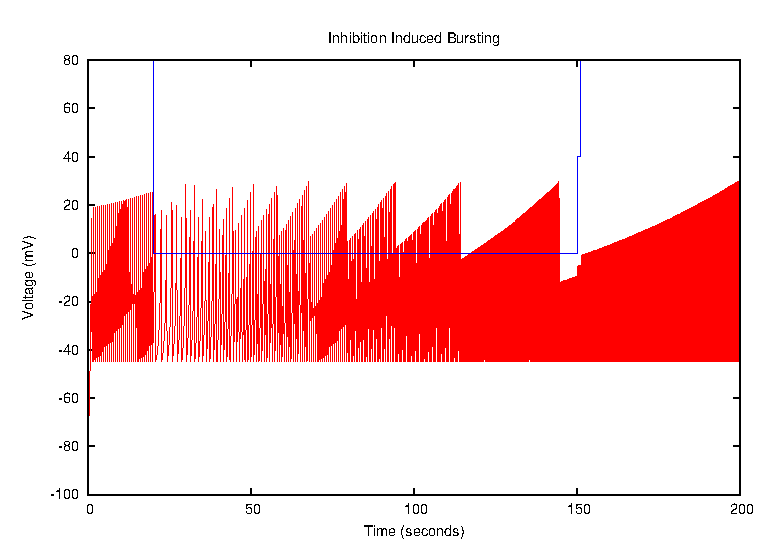
\epsfig{file=data/figures/T,width=14cm,height=8cm}
\end{center}
\caption{\label{pict20}Inhibition Induced Bursting, with $I$ in blue}
\end{figure}

Though I would consider the spiking pattern generated during inhibition to be a burst, I don't know if I'd consider it to be a periodic bursting pattern. I could answer this question by letting the simulation run a bit longer, though I'd like to have more control over how localized the bursts are and how often they come. 

\vspace{2mm}

Still, I was more satisified with this result than I was with the Rebound Spike pattern, as I felt this was a neater result. 

\vfil\eject

{\bf Conclusions}
\bigskip

As I stated in the introduction, the firing patterns were replicated with varying degrees of success. In the end I did everything to do replicate the results obtained by Izhikevich. With that in mind I chose to switch between Euler and Runge-Kutta where I saw it fit. I also changed the parameters outlined in his code if they were not producing results I liked. 

\vspace{2mm}

In terms of simulation methods and time step selection, I found that the majority of my replications were best carried out using sloppier methods with larger time steps. Every plot included in this report was using a timestep of 1, and there were only a few cases where I found RK4 to be a better replication of Izhikevich's results. 

\vspace{2mm}

The problem I have mentioned earlier regarding the ``localization'' of spikes was somewhat remedied when a smaller timestep was used. However, in the cases where I really needed this (i.e rebound bursting) I lost the rebound effect; I could in theory get this back by changing some parameters, but there were a number of patterns (like Tonic Bursting and Inhibition-Induced potentials) where the smaller time step made the data look quite bizarre. 

\vspace{2mm}

The complete output data for $DT=1$ and $DT=0.1$ are included with this report in the folders \begin{verbatim}data/figures/one\end{verbatim} and \begin{verbatim}data/figures/oneTenth\end{verbatim}. 

\end{document}
